
\documentclass[conference]{IEEEtran}
\usepackage{cite}
\usepackage{graphicx}
\usepackage{amsmath}
\usepackage{enumerate}
\usepackage{xcolor}
\usepackage{pgfplots}
\usepackage{tikz}
\usepackage{listings}
\usepackage[linesnumbered]{algorithm2e}
\usepackage{tikz}

\definecolor{bblue}{HTML}{4F81BD}
\definecolor{rred}{HTML}{C0504D}
\definecolor{ggreen}{HTML}{9BBB59}
\definecolor{ppurple}{HTML}{9F4C7C}

% correct bad hyphenation here
\hyphenation{op-tical net-works semi-conduc-tor}

\pgfplotsset{grid style={dashed,gray}}

\begin{document}

\title{PRECINCT:\@ An Incremental Approach for Preventing Clone Insertion at Commit Time}


\author{\IEEEauthorblockN{Mathieu Nayrolles, }
\IEEEauthorblockA{Software Behaviour Analysis (SBA) Research Lab\\
ECE, Concordia University\\
Montreal, Canada\\
m\_nayrol@ece.concordia.ca}
\and
\IEEEauthorblockN{Abdelwahab Hamou-Lhadj}
\IEEEauthorblockA{Software Behaviour Analysis (SBA) Research Lab\\
ECE, Concordia University\\
Montreal, Canada\\
abdelw@ece.concordia.ca}}

% make the title area
\maketitle

% As a general rule, do not put math, special symbols or citations
% in the abstract
\begin{abstract}
Software clones are considered harmful since they may cause the same buggy code to appear in multiple places in the code, making software maintenance and evolution tasks challenging. Clone detection has been an active research field for almost two decades.
Interestingly, most existing techniques focus on detecting clones after they are inserted in the code.
In this paper, we take another look at the clone detection problem by designing a novel approach for preventing the insertion of clones in the first place. Our approach, called PRECINCT (PREventing Clones INsertion at Commit Time),  detects efficiently Type 3 software clones at commit time by means of pre-commit hooks.
This way, changes to the code are analysed and suspicious clones are flagged before they reach the central code repository in the version control system.  The application of PRECINCT to three systems developed independently shows that PRECINCT can prevent the insertion of up to 97.7\% of the clones at commit.


\end{abstract}


\IEEEpeerreviewmaketitle

\section{Introduction}
\label{sec:Introduction}


Code clones appear when developers reuse code with little to no modification to the original code.
Studies have shown  that clones can account for about 7\% to 50\% of code in a given software system\cite{Baker, StephaneDucasse}.
Developers often reuse code (and create clones) in their software on purpose\cite{Kim2005}.
Nevertheless, clones are considered a bad practice in software development since they can introduce new bugs in the code\cite{Kapser2006,Juergens2009,Li2006}.
If a  bug is discovered in one segment of the code that has been copied and pasted several times, then the developers will have to remember the places where this segment has been reused in order to fix the bug in each place.

In the last two decades, there have been many studies and tools that aim at detecting clones. They can be grouped into three categories.
The first category includes techniques that treat the source code as text and use transformation and normalization methods to compare various code fragments\cite{Johnson1994,Johnson1993, Cordy2011, Roy2008}.
The second category includes methods that
use lexical analysis, where the source code is sliced into sequences of tokens, similar to the way a compiler operates\cite{Baker,Bakera,Baker2002,Kamiya2002,Li2006}.
The tokens are used to compare code fragments.
Finally, syntactic analysis has also been performed where the source code is converted into trees, more particularly abstract syntax tree (AST), and then the clone detection is performed using tree matching algorithms\cite{Baxter1998, Komondoor2000, Tairas2006, Falke2008}.

Although these techniques and tools have been shown to be useful in detecting clones, they operate offline (i.e., after the clones have been inserted). Software developers might be reluctant to use these tools on a day-to-day basis (i.e., as part of the continuous development process), unless they are involved in a major refactoring effort. This problem is somehow similar to the problem of adopting bug identification tools. Johnson et al. \cite{Johnson2013} showed that these tools are challenging to use because they do not integrate well with the day-to-day workflow of a developer. Also they output a large amount of data when applied to the entire system, making it hard to understand and analyse their results.

In this paper, we present PRECINCT (PREventing Clones INsertion at Commit Time) that focuses on preventing the insertion of clones at commit time, i.e., before they reach the central code repository. PRECINCT is an online clone detection technique that relies on the use of pre-commit hooks capabilities of modern source code version control systems. A pre-commit hook is a process that one can implement to receive the latest modification to the source code done by a given developer just before the code reaches the central repository.
PRECINCT intercepts this modification and analyses its  content to see whether a suspicious clone has been introduced or not.
A flag is raised if a code fragment is suspected to be a clone of an existing code segment.
In fact, PRECINCT, itself, can be seen as a pre-commit hook that detects clones that might have been inserted in the latest changes with regard to the rest of the source code.
This said, only a fraction of the code is analysed, making PRECINCT efficient compared to leading  clone detection techniques such as NICAD (Accurate Detection of Near-miss Intentional Clones) \cite{Cordy2011}.
Moreover, the detected clones are presented using a classical `diff' output that developers are familiar with.
PRECINCT is also well integrated with the workflow of the developers since it is used in conjunction with a source code version control systems such as Git\footnote{https://git-scm.com/}.

%[WAHAB: YOU NEED TO ADD A PARAGRAPH TALKING ABOUT CLONE TYPES AND MAKING THE CASE FOR TYPE 3-1, WHILE EXPLAINING THAT PRECINCT FOCUSES ON TYPE 3-1]

Many taxonomies have been published in an attempt to classify clones into types. \cite{Mayrand1996,Balazinska1999,Koschke2006,Bellon2007,NeilDavey,Kontogiannis,Kapser}.
Despite the particularities of each proposed taxonomy, researchers agree to the following classification.
Type 1 clones are copy-pasted blocks of code that only differ from each other in terms of non-code artefacts such as indentation, whitespaces, comments and so on.
Type 2 clones are blocks of code that are syntactically identical at the exception of literals, identifiers and types that can be modified.
In addition, Type 2 also shares the particularities of Type 1 about indentation, whitespaces and comments.
Type 3 clones are similar to Type 2 clones in terms of modification of literals, identifiers, types, indentation, whitespaces and comments but also contain added or deleted code statements.
Finally, Type 4 are code blocks that perform the same tasks, but using a completely different implementation.

In this study, we focus on Type 3 clones as they are more challenging to detect. Since Type 3 clones include Type 1 and 2 clones, then these types could also be detected by PRECINCT as well.

We evaluated the effectiveness of PRECINCT using precision and recall on three systems, developed independently and written in both C and Java. The results show that PRECINCT prevents Type 3 clones to reach the source version system with an average accuracy of 97.7\%.

The rest of this paper is organized as follows: In Section~\ref{sec:Related Work}, we present the studies related to PRECINCT. Then, in Section~\ref{sec:The PRECINCT Approach}, we present the PRECINCT approach. The evaluation of PRECINCT is the subject of  Section~\ref{sec:Experimentations}, followed by threats to validity.
Finally, we conclude the paper in Section~\ref{sec:Conclusion}.

\section{Related Work}
\label{sec:Related Work}

Clone detection is an important and difficult task. Throughout the years, researchers and practitioners have developed a considerable number of methods and tools in order to detect efficiently source code clones.

Text-based techniques use the code --- often raw (e.g. with comments) --- and compare sequences of code (blocks) to each other in order to identify potential clones. Johnson was perhaps the first one to use fingerprints to detect clones\cite{Johnson1993,Johnson1994}. Blocks of code are hashed, producing fingerprints that can be compared.
If two blocks share the same fingerprint, they are considered as clones.
Manber et al. \cite{Manber1994} and Ducasse et al.\cite{Ducasse1999} refined the fingerprint technique by using leading keywords and dot-plots.

Tree-matching and metric-based are two sub-categories of syntactic analysis for clone detection.
Syntactic analysis consists of building abstract syntax trees (AST) and analyse them with a set of dedicated metrics or searching for identical sub-trees.
Many approaches using AST have been published using sub-tree comparison including the work of Baxter et al.\cite{Baxter1998}, Wahleret et al. \cite{Wahler}, or more recently, the work of Jian et al. with Deckard \cite{Jiang2007}.
An AST-based approach compares metrics computed on the AST, rather than the code itself, to identify clones \cite{Patenaude1999, Balazinska}.

Another approach to detect clones is to use static analysis and to leverage the semantics of the program to improve the detection.
These techniques rely on program dependency graphs where nodes are statements and edges are dependencies.
Then, the problem of finding clones is reduced to the problem of finding identical sub-groups in the program dependency graph.
Examples of recent techniques that fall into this category are the ones presented by Krinke et al.\cite{Krinke2001} and  Gabel et al. \cite{Gabel2008}.

Many clone detection tools have been created using a lexical approach for clone detection. Here, the code is transformed into a series of tokens. If sub-series repeat themselves, it means that a potential clone is in the code. Some popular tools that use this technique include, but not limited to, Dup\cite{Baker}, CCFinder\cite{Kamiya2002}, and CP-Miner\cite{Li2006}.

Furthermore, a large number of taxonomies have been published in an attempt to classify  clones and ease the research on clone detection\cite{Mayrand1996,Balazinska1999,Koschke2006,Bellon2007,NeilDavey,Kontogiannis,Kapser}.

Other active research activities in clone detection focus on clone removal and management. Once detected, an obvious step is to provide approaches to remove clones in an automatic way or (at least) keep track of them if removing them is not an option.
Most modern IDEs provide the \textit{extract method} feature that transforms a potentially copy-pasted block of code into a method and a call to the newly generated method\cite{Komondoor,higo2004refactoring}.
More advanced techniques (see Codelink\cite{Toomim} and\cite{Duala-Ekoko2007}) involve analysing the output of CCFinder\cite{Bomarius2004} or program dependencies graphs\cite{higo2004refactoring} to automatically suggest a method that would go through the \textit{extract method} process.

The aforementioned  techniques, however, focus on detecting clones after they are inserted in the code. Only a few studies focus on preventing the insertion of clones. Lague et al. \cite{Lague} conducted a very large empirical study with 10,000 developers over 3 years, where developers where asked to use clone detection tools during the development process of a very large telecom system. The authors found that while clones are being removed over time, using clone detection tools help improving the quality of the system as it prevents defects to reach the customers. Duala et al. \cite{Duala-Ekoko2007,Duala-Ekoko2010} proposed to create clone region descriptors (CRDs), which describe clone regions within methods in a robust way that is independent from the exact text of the clone region or its location in a file. Then, using CRDs, clone insertion can be prevented.

PRECINCT aims to prevent clone insertion while integrating the clone detection process in a transparent manner in the day-to-day development process. This way, software developers do not have to resort to external tools to remove clones after they are inserted. Our approach operates at commit time, notifying software developers of possible clones as they commit their code.


\section{The PRECINCT Approach}
\label{sec:The PRECINCT Approach}

\begin{figure*}
  \centering
    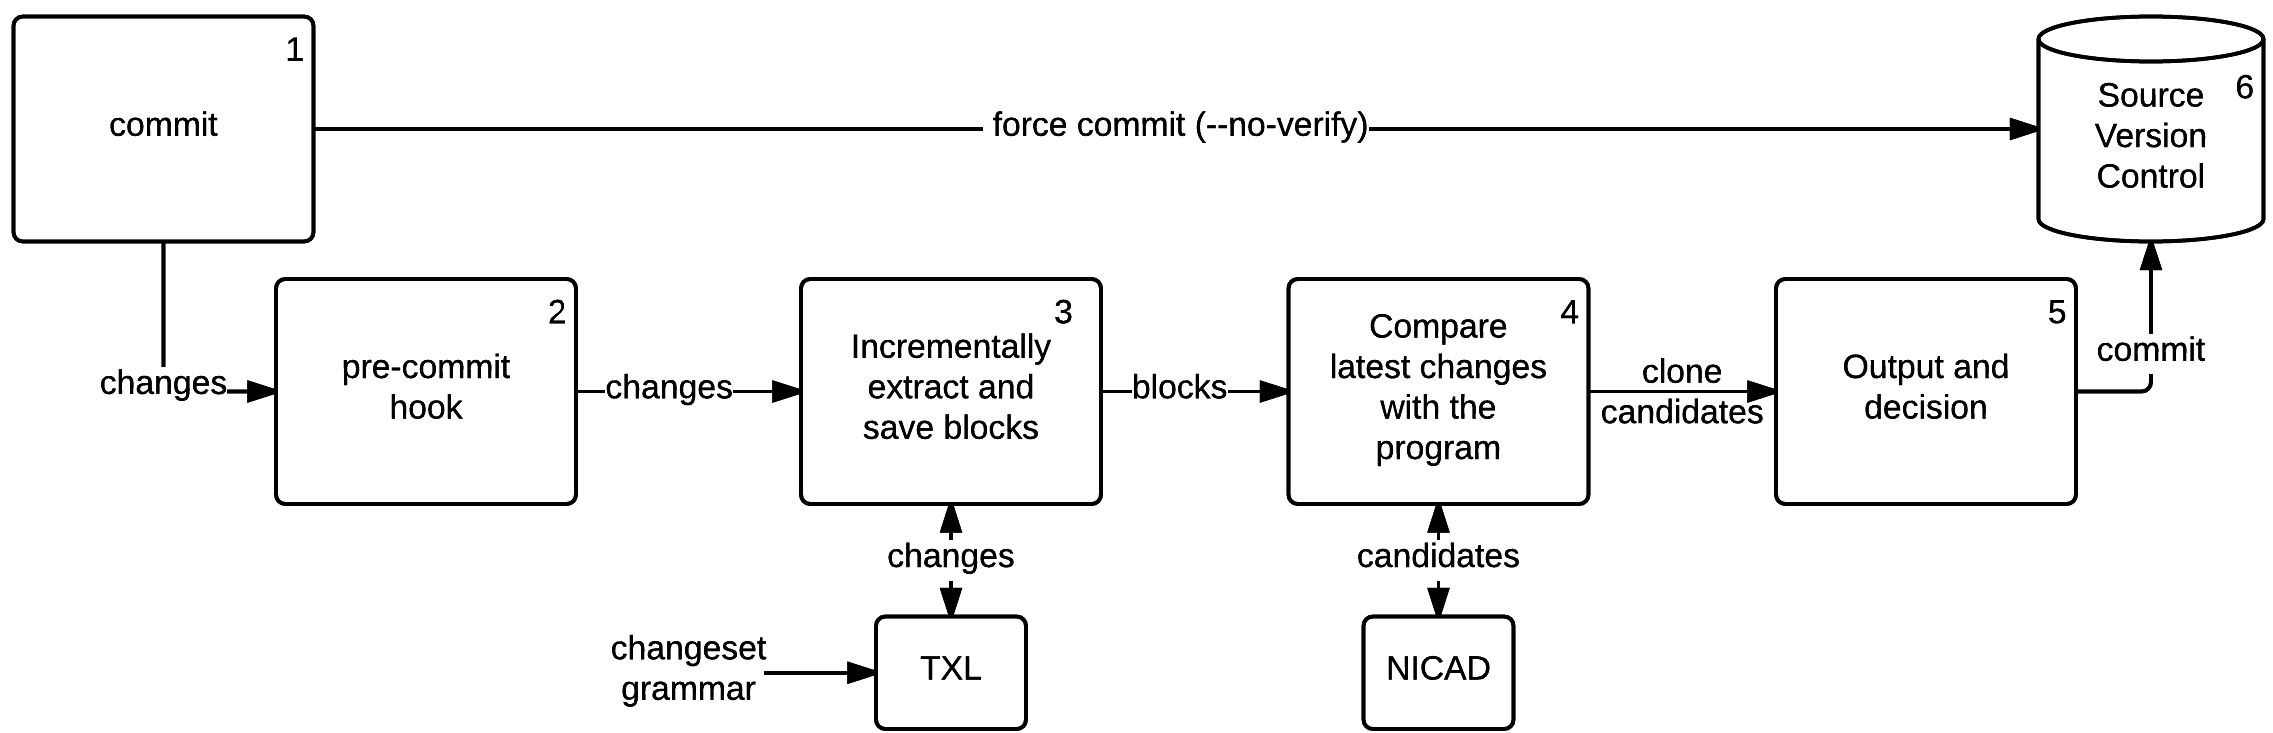
\includegraphics[width=\textwidth]{media/approach.png}
    \caption{ Overview of the PRECINCT Approach.\label{fig:precinct-approach}}
\end{figure*}

The PRECINCT approach is composed of six steps.
The first two steps are part of the developer workflow.
Indeed, the first step is the commit step where developers send their latest changes to the central repository and the last step is the reception of the commit by the central repository.
The second step is the pre-commit hook, which kicks in as the first operation when one wants to commit.
The pre-commit hook has access to the changes in terms of files that have been modified, more specifically, the lines that have been modified. The modified lines of the files are sent to TXL\cite{Cordy2006a} for block extraction. Then, the blocks are compared to previously extracted blocks in order to identify candidate clones using the comparison engine of NICAD\cite{Cordy2011}. We chose NICAD engine because it has been shown to provide high accuracy \cite{Cordy2011}. The tool is also readily available, easy to use, customizable, and works with TXL. Note, however, that PRECINCT can also work with other engines for comparing code fragments.
Finally, the output of NICAD is further refined and presented to the user for a decision round.
These steps are discussed in more detail in the following subsections.

\subsection{Commit}
\label{sub:Commit}

In version control systems, a commit adds the latest changes made to the source code to the repository, making these changes part of the head revision of the repository.
Commits in version control systems are kept in the repository indefinitely. Thus, when other users do an update or a checkout from the repository, they will receive the latest committed version, unless they wish to retrieve a previous version of the source code in the repository.
Version control systems allow rolling back to previous versions easily.
In this context, a commit within a version control system is protected as it is easily rolled back, even after the commit has been done.

\subsection{Pre-Commit Hook}
\label{sub:Pre-Commit Hook}

Hooks are custom scripts set to fire off when certain important actions occur.
There are two groups of  hooks: client-side and server-side.
Client-side hooks are triggered by operations such as committing and merging, whereas server-side hooks run on network operations such as receiving pushed commits.
These hooks can be used for all sorts of reasons such as compliance to coding rules or automatic run of unit test suites.


The pre-commit hook is run first, before one even types in a commit message. It is used to inspect the snapshot that is about to be committed.
% Exiting [WAHAB: I DO NOT UNDERSTAND THIS SENTENCE] non-zero from this hook aborts the commit, although one can bypass it with a no-verify commit (a feature that exists in Git and other version systems).
Depending on the exit status of the hook, the commit will be aborted and not pushed to the central repository.
Also, developers can choose to ignore the pre-hook. In Git, for example, they will need to use the command \texttt{git commit --no-verify} instead of \texttt{git commit}.
This can be useful in case of an urgent need for fixing a bug where the code has to reach the central repository as quickly as possible.
Developers can do things like check for code style (run lint or something equivalent), check for trailing white spaces (the default hook does exactly this), or check for appropriate documentation on new methods.

PRECINCT is a set of bash scripts where the entry point of these scripts lies in the pre-commit hooks. Pre-commit hooks are easy to create and implement as depicted in Listing~\ref{gitprehook}.
This pre-hook is shipped with Git, a popular version control system.
Note that even though we use Git as the main version control to present PRECINCT, we believe that the techniques presented in this paper are readily applicable to other version control systems.
In Listing~\ref{gitprehook}, from lines 3 to 11, the script identifies if the commit is the first one in order to select the revision to work against.
Then, in Lines 18 and 19, the script checks for trailing whitespace and fails if any are found.

For PRECINCT to work, we just have to add the call to our script suite instead or in addition of the whitespace check.

\noindent\begin{minipage}{0.90\linewidth}

  \lstinputlisting[language=Bash, firstnumber=1, numbers=right, stepnumber=1,leftmargin=30, label=gitprehook, caption=Git Pre-Commit Hook Sample]{media/pre-commit.sample}

\end{minipage}


\subsection{Extract and Save Blocks}
\label{sub:Extract and Save Blocks}

A block is a set of consecutive lines of code that will be compared to all other blocks in order to identify clones.
To achieve this critical part of PRECINCT, we rely on TXL\cite{Cordy2006a}, which is a first-order functional programming over linear term rewriting, developed by Cordy et al.\cite{Cordy2006a}.
For TXL to work, one has to write a grammar describing the syntax of the source  language and the transformations needed. TXL has three main phases: \textit{parse, transform}, \textit{unparse}.
In the parse phase, the grammar controls not only the input but also the output form.
Listing~\ref{txlsample} --- extracted from the official documentation\footnote{http://txl.ca} --- shows a grammar matching an \textit{if-then-else} statement in C with some special keywords: [IN] (indent), [EX] (exdent) and [NL] (newline) that will be used for the output form.

\noindent\begin{minipage}{0.90\linewidth}

  \lstinputlisting[language=Bash, firstnumber=1, numbers=right, stepnumber=1,leftmargin=30, label=txlsample, caption=Txl Sample Sample]{media/txl.sample}

\end{minipage}

Then, the \textit{transform} phase will, as the name suggests, apply transformation rules that can, for example, normalize or abstract the source code. Finally, the third phase of TXL,  called \textit{unparse}, unparses the transformed parsed input in order to output it.
Also, TXL supports what the creators call Agile Parsing\cite{Dean}, which allow developers to redefine the rules of the grammar and, therefore, apply different rules than the original ones.


PRECINCT takes advantage of that by redefining the blocks that should be extracted for the purpose of clone comparison, leaving out the  blocks that are out of scope.
More precisely, before each commit, we only extract the blocks belonging to the modified parts of the source code.
Hence, we only process, in an incremental manner, the latest modification of the source code instead of the source code as a whole.

We have selected TXL for several reasons. First, TXL is easy to install and to integrate with the normal workflow of a developer.
Second, it was relatively easy to create a grammar that accepts commits as input.
This is because TXL is shipped with C, Java, Csharp, Python and WSDL grammars that define all the particularities of these languages, with the ability to customize these grammars to accept changesets (chunks of the modified source code that include the added, modified, and deleted lines) instead of the whole code.

Algorithm~\ref{alg:extract} presents an overview of the ``extract" and ``save" blocks operations of PRECINCT. This algorithm receives as arguments, the changesets, the blocks that have been previously extracted and a boolean named compare\_history.
Then, from Lines 1 to 9 lie the $for$ loop that iterates over the changesets. For each changeset (Line 2), we extract the blocks by calling the $~extract\_blocks(Changeset~cs)$ function.
In this function, we expand our changeset to the left and to the right in order to have a complete block.
As depicted by Listing~\ref{commitsample}, changesets contain only the modified chunk of code and not necessarily complete blocks. Indeed, we have a block from Line 3 to Line 6 and deleted lines from Line 8 to 14.
However, in Line 7 we can see the end of a block, but we do not have its beginning. Therefore, we need to expand the changeset to the left in order to have syntactically correct blocks.
We do so by checking the block's beginning and ending (using \{ and \}) in C for example.
Then, we send these expanded changesets to TXL for block extraction and formalization.

\begin{algorithm}
 \KwData{$Changeset[]$ changesets\;
 $Block[]$ prior\_blocks\;
 $Boolean$ compare\_history\;
 }
 \KwResult{Up to date blocks of the systems}
 \For{$i \leftarrow 0$ \KwTo$size\_of~changesets$}{
    Block[] blocks $\leftarrow$ $extract\_blocks(changesets)$\;
    \For{$j \leftarrow 0$ \KwTo$size\_of~blocks$}{
       \If{not $compare\_history$ AND $blocks[j]$ overrides one of $prior\_blocks$}{
          delete $prior\_block$\;
       }
       write $blocks[j]$\;
    }
 }

 \SetKwProg{myproc}{Function}{ $~extract\_blocks(Changeset~cs)$}{}
   \myproc{\proc{}}{

   \uIf{$cs~is~unbalanced~right$}{$cs \leftarrow expand\_left(cs)$\;}

   \ElseIf{$cs~is~unbalanced~left$}{$cs \leftarrow expand\_right(cs)$\;}

   \nl\KwRet$txl\_extract\_blocks(cs)$\;
   }


 \caption{Overview of the Extract Blocks Operation\label{alg:extract}}
\end{algorithm}

\noindent\begin{minipage}{0.90\linewidth}

  \lstinputlisting[language=Bash, firstnumber=1, numbers=right, stepnumber=1,leftmargin=30, label=commitsample, caption=Changeset c4016c of monit]{media/commit.sample}

\end{minipage}



For each extracted block, we check if the current block overrides (replaces) a previous block (Line 4).
In such a case, we delete the previous block as it does not represent the current version of the program anymore (Line 5).
Also, we have an optional step in PRECINCT defined in Line 4. The compare\_history is a condition to delete overridden blocks.

% [WAHAB: I DON'T UNDERSTAND THE FOLLOWING 3 SENTENCES. PLEASE REPHRASE]
We believe that deleted blocks have been deleted for a good reason (bug, default, removed features, \ldots) and if a newly inserted block matches an old one, it could be worth knowing in order to improve the quality of the system at hand.
This feature is deactivated by default.

In summary, this step receives the files and lines, modified by the latest changes made by the developer and produces an up to date block representation of the system at hand in an incremental way.
The blocks are analysed in the next step to discover potential clones.

\subsection{Compare Extracted Blocks}
\label{sub:Compare Extracted Blocks}

In order to compare the extracted blocks and detect potential clones, we can only resort to text-based techniques.
This is because lexical and syntactic analysis approaches (alternatives to text-based comparisons) would require a complete program to work, a program that compiles.
In the relatively wide-range of tools and techniques that exist to detect clones by considering code as text\cite{Johnson1993,Johnson1994,Marcus,Manber1994,StephaneDucasse,Wettel2005}, we selected NICAD as the main text-based method for comparing clones \cite{Cordy2011} for several reasons.
First, NICAD is built on top of TXL, which we also used in the previous step.
Second, NICAD is able to detect all Types 1, 2 and 3 software clones.

NICAD  works in three phases: \textit{Extraction}, \textit{Comparison} and \textit{Reporting}. During the \textit{Extraction} phase all potential clones are identified, pretty-printed, and extracted.
We do not use the \textit{Extraction} phase of NICAD as it has been built to work on programs that are syntactically correct, which is not the case for changesets.
We replaced NICAD's \textit{Extraction} phase with our own scripts, described in the previous section.

In the \textit{Comparison} phase, extracted blocks are transformed, clustered and compared in order to find potential clones.
Using TXL sub-programs, blocks go through a process called pretty-printing where they are stripped of formatting and comments.
When code fragments are cloned, some comments, indentation or spacing are changed according to the new context where the new code is used. This pretty-printing process ensures that all code will have the same spacing and formatting, which renders the comparison of code fragments easier.
Furthermore, in the pretty-printing process, statements can be broken down into several lines.
Table~\ref{tab:pretty-printing} shows how this can improve the accuracy of clone detection with three \texttt{for} statements, \texttt{ for (i=0; i<10; i++)}, \texttt{for (i=1; i<10; i++)} and \texttt{ for (j=2; j<100; j++)}.
The pretty-printing allows NICAD to detect Segments 1 and 2 as a clone pair because only the initialization of $i$ changed.
This specific example would not have been marked as a clone by other  tools we tested such as Duploc\cite{Ducasse1999}.
In addition to the pretty-printing, code can be normalized and filtered to detect different classes of clones and match user preferences.

\begin{table}[]
\centering
\caption{Pretty-Printing Example\cite{Iss2009}}
\label{tab:pretty-printing}
\resizebox{0.5\textwidth}{!}{%
\begin{tabular}{l|l|l|l|l|l}
Segment 1          & Segment 2          & Segment 3           & S1 \& S2 & S1 \& S3 & S2 \& S3 \\ \hline \hline
for (              & for (              & for (               & 1        & 1        & 1        \\
i = 0;             & i = 1;             & j = 2;              & 0        & 0        & 0        \\
i \textgreater 10; & i \textgreater 10; & j \textgreater 100; & 1        & 0        & 0        \\ 
i++)               & i++)               & j++)                & 1        & 0        & 0        \\ \hline \hline
\multicolumn{3}{c|}{Total Matches}                            & 3        & 1        & 1        \\ \hline
\multicolumn{3}{c|}{Total Mismatches}                         & 1        & 3        & 3
\end{tabular}
}
\end{table}


Finally, the extracted, pretty-printed, normalized and filtered blocks are marked as potential clones using a Longest Common Subsequence (LCS) algorithm\cite{Hunt1977}. Then, a percentage of unique statements can be computed and, depending on a given threshold (see Section~\ref{sec:Experimentations}), the blocks are marked as clones.

The last step of NICAD, which acts as our clone comparison engine, is the \textit{reporting}. However, to prevent PRECINCT from outputting a large amount of data (an issue that many clone detection techniques face), we  implemented our own reporting system, which is also well embedded with the workflow of developers. This reporting system is the subject of the next section.

As a summary, this step receives potentially expanded and balanced blocks from the extraction step.
Then, the blocks are pretty-printed, normalized, filtered and fed to an LCS algorithm in order to detect potential clones.
Moreover, the clone detection in PRECINCT is less intensive than NICAD because we only compare the latest changes with the rest of the program instead of comparing all the blocks with each other.

\subsection{Output and Decision}
\label{sub:Output and Decision}

In this final step, we report the result of the clone detection at commit time with respect to the latest changes made by the developer. The process is straightforward. Every change made by the developers goes through the previous steps and checked for the introduction of potential clones. For each file that is suspected to contain a clone, one line is printed to the command line with the following options: (I) Inspect, (D) Disregard, (R) Remove from the commit as shown by Figure \ref{fig:hook}. In comparison to this simple and interactive output, NICAD outputs each and every detail of the detection result such as the total number of potential clones, the total number of lines, the total number of unique line text chars, the total number of unique lines, and so on. We think that so many details might make it hard for developers to react to these results. A problem that was also raised by Johnson et al. \cite{Johnson2013}.
Then the potential clones are stored in XML files that can be viewed using an Internet browser or a text editor.

\begin{figure}
  \centering
    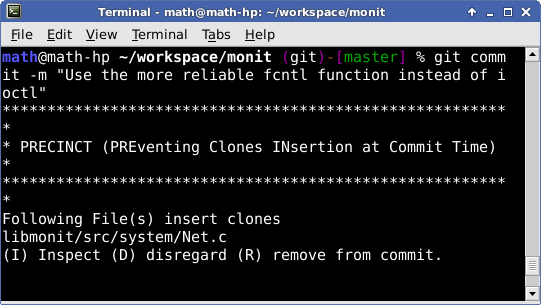
\includegraphics[width=0.5\textwidth]{media/commit.png}
    \caption{PRECINCT output when replaying commit \texttt{710b6b4} of monit.\label{fig:hook}}
\end{figure}

(I) Inspect will cause a diff-like visualization of the suspected clones while (D) disregard will simply ignore the finding.
To integrate PRECINCT in the workflow of the developer we also propose the  remove option (R). This option will simply remove the suspected file from the commit that is about to be sent to the central repository.
Also, if the user types an option key twice, e.g., II, DD or RR, then the option will be applied to all files.
For instance, if the developer types DD at any point, the PRECINCT's results will be disregarded and the commit will be allowed to go through. We believe that this simple mechanism will encourage developers to use PRECINCT like they would use any other feature of Git (or any other control version system).



\section{Experimentations}
\label{sec:Experimentations}

In this section, we show the effectiveness of PRECINCT for
detect clones at commit time in three open source systems\footnote{The programs used and instructions to reproduce the experiments are made available for download from https://research.mathieu-nayrolles.com/precinct/}.

The aim of the case study is to answer the following question: \textit{Can we detect clones at commit time, i.e., before they are inserted in the final code, if so, what would be the accuracy compared to a traditional clone detection tool such as NICAD?}

\subsection{Target Systems}
\label{sub:Target Systems}

Table~\ref{tab:sut} shows the systems used in this study and their characteristics in terms of the number files they contain and the size in KLoC (Kilo Lines of Code). We also include the number of revisions used for each system and the programming language in which the system is written.

\begin{table}[]
\centering
\caption{List of Target Systems in Terms of Files and Kilo Line of Code (KLOC) at current version and Language}
\label{tab:sut}
\resizebox{0.5\textwidth}{!}{%
\begin{tabular}{c|c|c|c|c}
SUT        & Revisions & Files & KLoC & Language \\ \hline\hline
Monit      & 826       & 264   & 107  & C        \\ \hline
Jhotdraw   & 735       & 1984  & 44   & Java     \\ \hline
dnsjava    & 1637      & 233   & 47   & Java     \\ \hline
\end{tabular}
}
\end{table}

Monit\footnote{https://mmonit.com/monit/} is a small open source utility for managing and monitoring Unix systems.
Monit is used to conduct automatic maintenance and repair and supports the ability to identify causal actions to detect errors.
This system is written in C and composed of 826 revisions, 264 files, and the latest version has 107 KLoC.
We have chosen Monit as a target system because it was one of the systems NICAD was tested on.

JHotDraw\footnote{http://www.jhotdraw.org/} is a Java GUI framework for technical and structured graphics.
It has been developed as a ``design exercise''. Its design relies heavily on the use of design patterns. JHotDraw is composed of 735 revisions, 1984 files, and the latest revision has 44 KLoC. It is written in Java and it is often used by researchers as a test bench. JHotDraw was also used by NICAD's developers to evaluate their approach.

Dnsjava\footnote{http://www.dnsjava.org/} is a tool for implementing the DNS (Domain Name Service) mechanisms in Java.
This tool can be used for queries, zone transfers, and dynamic updates.
It is not as large as the other two, but it still makes an interesting case subject because it has been well maintained for the past decade. Also, this tool is used in many other popular tools such as Aspirin, Muffin and
Scarab. Dnsjava is composed of 1637 revisions, 233 files, the latest revision contains 47 KLoC.
We have chosen this system because we are familiar with it as we used it before\cite{Nayrolles2015c}.

\subsection{Process}
\label{sub:Process}


Figure \ref{fig:precinct-branching} shows the process we followed to validate the effectiveness of PRECINCT.

\begin{figure}
  \centering
    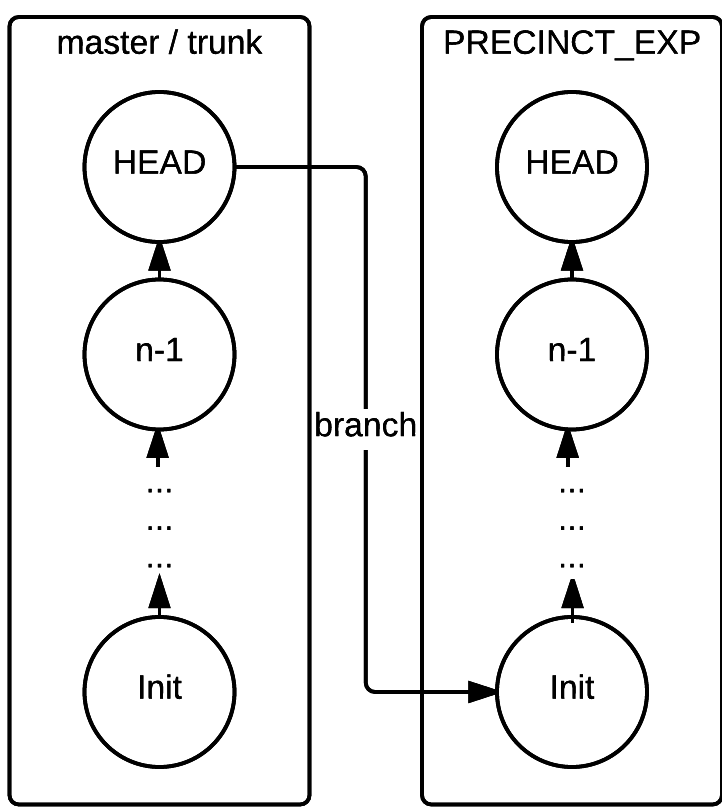
\includegraphics[width=0.3\textwidth]{media/branch.png}
    \caption{PRECINCT Branching.\label{fig:precinct-branching}}
\end{figure}

As our approach relies on commit pre-hooks to detect possible clones during the development process (more particularly at commit time), we had to find a way to \textit{replay} past commits. To do so, we  \textit{cloned} our test subjects, and then created a new branch called \textit{PRECINCT\_EXT}.
When created, this branch is reinitialized at the initial state of the project (the first commit) and each commit can be replayed as they have originally been. At each commit, we store the time taken for PRECINCT to run as well as the number of detected clone pairs. We also store the size of the output in terms of number of lines of text output by our method. The aim is to reduce the output size to help software developers interpret the results.

To validate the results obtained by PRECINCT, we needed to use a reliable clone detection approach to validate our results. For this, we use NICAD because of its popularity, high accuracy, and availability \cite{Cordy2011}, as we discussed before. This means, we run NICAD on the revisions of the system to obtain the clones. We use NICAD clones as a baseline for comparing the results obtained by PRECINCT.

It may appear strange that we are using NICAD to validate our approach, knowing that our approach uses NICAD's code comparison engine. In fact, what we are assessing here is the ability for PRECINCT to detect clones at commit time using changsets. The major part of PRECINCT is the ability to  intercept code changes and build working code blocks that are fed to a code fragment engine (in our case NICAD's engine). PRECINCT can be build on the top of any other code comparison engine.

We show the result of detecting Type 3 clones with a maximum line difference of 30\% as discussed in Table~\ref{tab:pretty-printing}. As discussed in the introductory section, we chose to report on Type 3 clones because they are more challenging to detect than Type 1 and 2. PRECINCT detects Type 1 and 2 too so does NICAD. For the time being, PRECINCT is not designed to detect Type 4 clones. These clones use different implementations. Detecting Type 4 clones is part of future work.

% [WAHAB: YOU NEED TO DEFINE PRECISION AND RECALL]

We assess the performance of PRECINCT in terms of precision (Equation 1) and recall (Equation 2).
Both precision and recall are computed by considering  NICAD's results as a baseline.
We also compute F$_{1}$-measure (Equation 3), i.e., the weighted average of precision and recall, to measure the accuracy of PRECINCT.

\begin{equation}
precision = \frac{|\{ NICAD_{detection} \} \cap \{ PRECINCT_{detection} \} |}{| \{ PRECINCT_{detection} \}|}
\end{equation}

\begin{equation}
recall = \frac{|\{ NICAD_{detection} \} \cap \{ PRECINCT_{detection} \} |}{| \{ NICAD_{detection} \}|}
\end{equation}

\begin{equation}
F_1-measure = 2 * \frac{precision * recall}{precision + recall}
\end{equation}


\begin {figure*}%[!hbtp]
\centering
\begin{tikzpicture}
    \begin{axis}[
      scale only axis, % The height and width argument only apply to the actual axis
    height=5cm,
    width=0.9\textwidth,
    grid = both,
    minor tick num=1,
    xlabel={Revisions},
    ylabel={Clones},
    xmin=0]
    \addplot table [smooth,blue,mark=none,x=revision,y=clones,col sep=comma] {data/monit};
    \addlegendentry{NICAD Detection}

    \addplot table [smooth,blue,mark=none,x=revision,y=prevented,col sep=comma] {data/monit};
    \addlegendentry{PRECINCT Detection}

    \addplot table [smooth,green,mark=none,x=revision,y=detected,col sep=comma] {data/monit};
    \addlegendentry{Remaining Clones}

    \end{axis}
    \end{tikzpicture}
    \caption{Monit clone detection over revisions\label{fig:r1}}
\end{figure*}

\begin {figure*}%[!hbtp]
\centering
\begin{tikzpicture}
    \begin{axis}[
      scale only axis, % The height and width argument only apply to the actual axis
    height=5cm,
    width=0.9\textwidth,
    grid = both,
    minor tick num=1,
    xlabel={Revisions},
    ylabel={Clones},
    xmin=0]
  \addplot table [smooth,red,mark=none,x=revision,y=clones,col sep=comma] {data/jhotdraw};
      \addlegendentry{NICAD Detection}

    \addplot table [smooth,green,mark=none,x=revision,y=detected,col sep=comma] {data/jhotdraw};
    \addlegendentry{PRECINCT Detection}

    \addplot table [smooth,red,mark=none,x=revision,y=prevented,col sep=comma] {data/jhotdraw};
    \addlegendentry{Remaining Clones}

    \end{axis}
    \end{tikzpicture}
    \caption{JHotDraw clone detection over revisions\label{fig:r2}}
\end{figure*}

\begin {figure*}%[!hbtp]
\centering
\begin{tikzpicture}
    \begin{axis}[
      scale only axis, % The height and width argument only apply to the actual axis
    height=5cm,
    width=0.9\textwidth,
    grid = both,
    minor tick num=1,
    xlabel={Revisions},
    ylabel={Clones},
    xmin=0]
  \addplot table [smooth,red,mark=none,x=revision,y=clones,col sep=comma] {data/dnsjava};
    \addlegendentry{NICAD Detection}

    \addplot table [smooth,green,mark=none,x=revision,y=detected,col sep=comma] {data/dnsjava};
    \addlegendentry{PRECINCT Detection}

    \addplot table [smooth,red,mark=none,x=revision,y=prevented,col sep=comma] {data/dnsjava};
    \addlegendentry{Remaining Clones}

    \end{axis}
    \end{tikzpicture}
    \caption{Dnsjava clone detection over revisions\label{fig:r3}}
\end{figure*}


\subsection{Results}
\label{sub:Results}

Figures~\ref{fig:r1},~\ref{fig:r2},~\ref{fig:r3} show the results of our study in terms of clone pairs that are detected per revision for our three subject systems: Monit, JHotDraw and Dnsjava. We compared our approach to NICAD that detects the clones after they are inserted. The blue line shows the clone detection performed by NICAD, the green line shows the clone detected by PRECINCT (again at commit time). The red line shows the clone pairs that have been missed by PRECINCT.

\begin{table*}[]
\centering
\caption{Overview of PRECINCT's results in terms of precision, recall, F$_{1}$-measure, execution time and output reduction.}
\label{tab:result}

\begin{tabular}{c|c|c|c|c|c||c|c}
         &  Detected & Precision & Recall & F1-measure & \begin{tabular}[c]{@{}c@{}}NICAD's Average\\ Execution Time\end{tabular} & \begin{tabular}[c]{@{}c@{}}PRECINCT's Average \\ Execution Time\end{tabular} & \begin{tabular}[c]{@{}c@{}}Overall \\ Output Reduction\end{tabular} \\ \hline\hline
Monit      & 123      & 96.1\%    & 100\%  & 98\%       & 2.2s                                                                     & 0.9s                                                                         & 88.3\%                                                              \\ \hline
JHotDraw   & 6490     & 98.3\%    & 100\%  & 99.1\%     & 5.1s                                                                     & 1.7s                                                                         & 70.1\%                                                              \\ \hline
DnsJava    & 226      & 82.8\%    & 100\%  & 90.6\%     & 1.8s                                                                     & 1.1s                                                                         & 88.6\%                                                              \\ \hline\hline
Total      & 6839     & 97.7\%    & 100\%  & 98.8\%     & 3s                                                                       & 1.2s                                                                         & 83.4\%                                                              \\ \hline
\end{tabular}

\end{table*}


Table~\ref{tab:result} summarizes PRECINCT's results in terms of precision, recall, F$_{1}$-measure, execution time and output reduction.
The first version of Monit contains 85 clone pairs and this number stays stable until Revision 100. From Revision 100 to 472 the detected clone pairs vary between 68 and 88 before reaching 219 at Revision 473.
The number of clone pairs goes down to 122 at Revision 491 and decreases to 128 in the last revision. PRECINCT was able to detect 96.1\% (123/128) of the clone pairs that are detected by NICAD with a 100\% recall.
It took in average around 1 second for PRECINCT to execute on a Debian 8 system with Intel(R) Core(TM) i5-2400 CPU @ 3.10GHz, 8Gb of DDR3 memory.
It is also worth mentioning that the computer we used is equipped with SSD (Solid State Drive).
This impacts the running time as clone detection is a file intensive operation.
Finally, the PRECINCT was able to output 88.3\% less lines than NICAD.

JHotDraw starts with 196 clone pairs at Revision 1 and reaches a pick of 2048 at Revision 180. The number of clones  continues to go up until Revisions 685 and 686 where the number of pairs is 1229 before picking at 6538 and more from Revisions 687 to 721.
PRECINCT was able to detect 98.3\% of the clone pairs detected by NICAD (6490/6599) with 100\% recall while executing on average in 1.7 second (compared to 5.1 seconds for NICAD).
With JHotDraw, we can clearly see the advantages of incremental approaches.
Indeed, the execution time of PRECINCT is loosely impacted by the number of files inside the system as the blocks are constructed incrementally.
Also, we only compare the latest change to the remaining of the program and not all the blocks to each other as NICAD.
We also were able to reduce by 70.1\% the number of lines output by NICAD.

Finally, for Dnsjava, the number of clone pairs starts high with 258 clones and goes up until Revision 70 where it reaches 165. Another quick drop is observed at Revision 239 where we found only 25 clone pairs. The number of clone pairs stays stable until Revision 1030 where it reaches 273. PRECINCT was able to detect 82.8\% of the clone pairs detected by NICAD (226/273) with 100\% recall, while executing on average in 1.1 second while NICAD took 3 seconds in average. PRECINCT outputs  83.4\% less lines of code than NICAD.

Overall, PRECINCT prevented 97.7\% of the 7000 clones (in all systems) to reach the central source code repository while executing more than twice as fast as NICAD (1.2 seconds compared to 3 seconds in average) while reducing the output in terms of lines of text output the developers by 83.4\% in average. Note here that we have not evaluate the quality of the output of PRECINCT compared to that out NICAD. We need to conduct user studies for this. We are however confident based on our own experience trying many clone detection tool, that a simpler and more interactive way to present the results of a clone detection tool is warranted.

The difference in execution time between NICAD and PRECINCT stems from the fact that, unlike PRICINCT, NICAD is not an incremental approach. For each revision, NICAD has to extract all the code blocks and then compares all the pairs with each other. On the other hand, PRECINCT only extracts blocks when they are modified and only compares what has been modified with the rest of the program.

The difference in precision between NICAD and PRECINCT (2.3\%)  can be explained by the fact that sometimes developers commit code that does not compile.
Such commits will still count as a revision, but TXL fails to extract blocks that do not comply with the target language syntax.
While NICAD also fails in such a case, the disadvantage of PRECINCT comes from the fact that the failed block is saved and used as reference until it is changed by a correct one in another commit.

\section{Threats to Validity}
\label{sec:Threats to Validity}

The selection of target systems is one of the common threats to validity for approaches aiming to improve the analysis of software systems.
It is possible that the selected programs share common properties that we are not aware of and therefore, invalidate our results.
However, the systems analysed by PRECINCT are the same as the ones used in similar studies.
Moreover, the systems  vary in terms of purpose, size and history.

In addition, we see a threat to validity that stems from the fact that we only used open source systems. The results may not be generalizable to industrial systems. We intend to undertake these studies in future work.

The programs we used in this study are all based on the Java, C and Python programming languages. This can limit the generalization of the results. However, similar to Java, C, Python, if one writes a TXL grammar for a new language --- which can be a relatively hard work --- then PRECINCT can work since PRECINT relies on TXL.

Finally, we use NICAD as the code comparison engine. The accuracy of NICAD affects the accuracy of PRECINCT. This said, since NICAD has been tested on large systems, we are confident that it is a suitable engine for comparing code using TXL. Also, there is nothing that prevents us from using other code comparisons engines, if need be.

In conclusion, internal and external validity have both been minimized by choosing a set of three different systems, using input data that can be found in any programming languages and version systems (commit and changesets).



\section{Conclusion}
\label{sec:Conclusion}

We presented PRECINCT (PREventing Clones INsertion at Commit Time), an incremental approach for preventing clone insertion at commit time that combines efficient block extraction and clone detection and integrate itself seamlessly in the day-to-day workflow of developers.
PRECINCT takes advantage of TXL and NICAD to create a clone detection tool approach that runs automatically before each commit in 1.2 second with a 97.7\% precision and a 100\% recall (when using NICAD results as a baseline).

Our approach also assesses two major factors that contribute to the slow adoption of clone detection tools: large number of data output by clone detection methods,  and  smooth integration with the task flow of the developers.
PRECINCT is able to reduce the number of lines output by a classical clone detection tool such as NICAD by 83.4\% while keeping all the necessary information that allow developers to decide whether the detect clone is in fact a clone.
Also, our approach is seamlessly integrated with the developers' workflow by means of pre-commit hooks, which are part any version control systems.

To build on this work, we need to experiment with additional (and larger) systems with the dual aim to (a) improve and fine-tune the approach, and (b) assess the scalability of our approach when applied to even larger (and proprietary) systems. Also, we want to improve PRECINCT to support Type 4 clones.


\bibliographystyle{IEEEtran}
\bibliography{library.bib}


\end{document}
